\setlength{\headheight}{15pt}
\lhead{\textbf{ITCS-6150}}
\chead{\textbf{Group 7}}
\rhead{\textbf{Final Report}}

\vspace{-2pt}

\begin{center}
    \begin{Large}
        \noindent\textbf{A Survey on the Limitations of Text Summarization Models}
    \end{Large}
\end{center}

\vspace{-10pt}

% Two column display for Team Members and Models & Datasets
\begin{multicols}{2}

    \begin{center}
        \begin{large}
            \noindent\textbf{Team Members}
        \end{large}
    \end{center}
    % Table of group members and their ids
    % Correct column widths for a table
    % 2 columns, 2 rows, no header
    \begin{center}
        \begin{tabular}{|lc|}
            \hline
            \textbf{David Gary} & \href{mailto:dgary9@uncc.edu}{801325583} \\ \hline
            \textbf{Michael Smalenberger} & \href{mailto:msmalenb@uncc.edu}{800984973} \\ \hline
            \textbf{Matthew Seman} & \href{mailto:mseman1@uncc.edu}{801156143} \\ \hline
            \textbf{Ryan Marsh} & \href{mailto:rmarsh4@uncc.edu}{800552800} \\ \hline
        \end{tabular}
    \end{center}

    \begin{center}
        \begin{large}
            \noindent\textbf{Models}
        \end{large}
    \end{center}

    \begin{center}
        \begin{tabular}{|lc|}
            \hline
            \href{https://github.com/zihangdai/xlnet}{XLNet Model\cite{XLNet}} & \href{https://huggingface.co/t5-base}{T5 Model\cite{T5}} \\ \hline
            \href{https://huggingface.co/facebook/bart-large-cnn}{BART Model\cite{BART}} &  \href{https://huggingface.co/facebook/bart-large-xsum}{BART-X Model\cite{BART}} \\ \hline
            \href{https://huggingface.co/google/pegasus-large}{Pegasus Model\cite{Pegasus}} &  \href{https://huggingface.co/google/pegasus-xsum}{Pegasus-X Model\cite{PegasusX}} \\ \hline
        \end{tabular}
    \end{center}


    \begin{center}
        \begin{large}
            \noindent\textbf{Sentiment Analysis Datasets}
        \end{large}
    \end{center}

    \begin{center}
        \begin{tabular}{|c|}
            \hline
            \href{https://paperswithcode.com/dataset/reddit-tifu}{Reddit TIFU Dataset\cite{RedditTIFU}} \\ \hline
            \href{https://paperswithcode.com/dataset/multi-news}{Multi-News Dataset\cite{Multinews}} \\ \hline
            \href{https://paperswithcode.com/dataset/s2orc}{S2ORC Dataset\cite{S2ORC}} \\ \hline
        \end{tabular}
    \end{center}

    \begin{center}
        \begin{large}
            \noindent\textbf{Summarization Datasets}
        \end{large}
    \end{center}

    \begin{center}
        \begin{tabular}{|c|}
            \hline
            \href{https://huggingface.co/datasets/gigaword}{Gigaword Dataset\cite{Gigaword1,Gigaword2}} \\ \hline
            \href{https://huggingface.co/datasets/cnn_dailymail}{CNN/DailyMail Dataset\cite{CNNDM}} \\ \hline
            \href{https://huggingface.co/datasets/xsum}{XSum Dataset\cite{XSumDataset}} \\ \hline
        \end{tabular}
    \end{center}

\end{multicols}

\vspace{5pt}

\begin{large}
    \noindent\textbf{Abstract}
\end{large}

\vspace{5pt}

The increasingly large volumes of text that must be consumed by people and businesses indicate that efficient, accurate, and reliable text summarizations is becoming crucial.
While artificial intelligence, and specifically intelligent systems continue to make progress in this field, a review of the relevant literature shows that the models these systems implement at times arrive at different conclusions.
Understanding why these differences exist, and when and how these differences should be mitigated are important questions that will facilitate future progress in this field.
To that end, this project report details the implementation of Rouge, Bleu, Jaccard Similarity, Perplexity, and Cosine Similarity which are commonly used text summarization scoring metrics.
Our tool implements six different state-of-the-art text summarization models, and allows for the user to select between these and various datasets, some of which correspond directly to our models' training data.
In this report, we discuss the limitations that can be easily seen by interacting with our text analysis tool.


\begin{large}
    \noindent\textbf{Introduction}
\end{large}

\vspace{5pt}

With the increase in the availability of data in many fields, the need for summarizing texts has become increasingly important.
Condensing large amounts of information into concise and consumable bits of information can have significant personal and business implications.
For example, helping readers parse through complex topics by reducing the information to its salient points can help individuals quickly apply new information and gain expertise.
Similarly, businesses have begun to use social media posts to gauge public sentiment toward cryptocurrencies in order to hedge their portfolios\cite{Crypto1, Crypto2}.
Wading through this enormous amount of information would not be possible without the ability to summarize posts and accurately gauge sentiment.

\vspace{5pt}

Artificial intelligence, and specifically Intelligent Systems (IS) using natural language processing (NLP), is increasingly used in order to accomplish this task. As progress continues to be made in developing and fine-tuning NLP applications for text summarization, there has become an increasing number of models available from which to choose.
These models are often created in order to accomplish a specific objective and are not intended to be highly effective in every scenario. Hence, when measuring the efficacy of different models, one may arrive at different conclusions.
While this does certainly not mean that one model is necessarily better than another, it is essential to understand what leads to these different outcomes.
Levels of efficacy when applied in different scenarios. 

\vspace{5pt}

When intelligent systems summarize text, they may arrive at different conclusions based on the model they implement.
For example, two methods of scoring are ROUGE\cite{Rouge} and Pyramid\cite{Pyramid}.
These two scoring systems produce different evaluations of the intelligent system.
In order to continue to make progress in this field, it is crucial to investigate what causes these evaluations to be different and why.


\vspace{5pt}

\begin{large}
    \noindent\textbf{Problem Statement}
\end{large}

Our system implements text analysis and summarization following the current standards of generalizability.
We make our platform available so that anyone can use it to summarize text or assess the tone of text either using several publicly available datasets implemented by our system or by the user loading a different dataset of their choice.
However, since the primary purpose of this project is to show the limitations of generalized text summarization models, the user should be aware that we do not strive to achieve perfect accuracy in summarization or sentiment analysis.
Instead, we highlight the differences of the models implemented, and therefore the majority of the remaining analysis and discussion will focus on these differences. 

\vspace{5pt}

\begin{large}
    \noindent\textbf{Literature Survey}
\end{large}

The main papers to form the foundation for our literature review is a paper by Guan et. al "A Survey on Automatic Text summarization in Transformer Models Applicability"\cite{Transformers}.
In this paper the authors conduct a survey of several models for text summarization.
Two main papers that informed our approach were a paper by Chin-Yew titled “ROUGE: How case for automatic evaluation of summaries”\cite{Rouge} and the paper by Nenkova, et al. titled “The Pyramid Method: Incorporating Human Content Selection Variation in Summarization Evaluation”\cite{Pyramid}.
These papers each present their own scoring metric for text summarization, but from the language of the original work, there are clear limitations to each metric's generalizability, despite the contradictory claims of wide-spread applicability made by the authors.
Our project implemented a scoring report that included the Rouge metric, but we did not utilize Pyramid as it seems to be falling out of favor in recent literature.
Instead, we implemented the BLEU and perplexity scoring metrics, along with the cosine similarity and Jaccard similarity comparitive metrics.
In this section, we will briefly explain what each of these metrics does and why they are useful for text summarization evaluation.

The Rouge score of a summary is broken down into three different scores: precision (P), recall (R), and F1 score (F) all under the Rouge-1 (unigram), Rouge-2 (bigram), and Rouge-L (longest common subsequence) scoring systems.
By providing this wide-range of n-gram approaches, Rouge gives a comprehensive view of the summary's performance.
Whether this is truly an accurate abstraction of the complexity of human language is debatable, but this is considered state-of-the-art in modern text summarization research.

The Bleu score is a metric that compares the n-grams of the reference summary to the n-grams of the generated summary.
In our implementation, the geometric mean of the Bleu precision scores for n-grams of length 1 through 4 is used, as this is fairly standard in the literature.
A more elaborate implementation might modify the n-gram lengths to reflect the percentile breakdown of n-grams in the reference summary, but this is not implemented in our tool.

The Jaccard similarity score compares the input text with the generated summary and returns a score between 0 and 1, where 1 is a perfect match.
The score is calculated by dividing the number of words that are in both the input text and the summary by the number of words that are in either the input text or the summary.
This is a useful score for extractive summarizations, but this score does very little to represent the effect of how words are rearranged in the summary.

The perplexity score we used for this project is different from how perplexity is considered in some other literature.
Instead, ours is a measure of how different in size the summarization is from the input text.
This metric is then mitigated by the summarization length constraints, and as a result, the metric outputs a probability of information loss.
It can be reasoned that this metric would be useful for both abstractive and extractive summarizations, but it has not yet been proven at this point and instead should guide the user to consider how much text has been cropped from the original input.

The cosine similarity score takes vectorized representations of the input text and the generated summary and returns a score between 0 and 1, where 1 is a perfect match.
The score is calculated by dividing the dot product of the two vectors by the product of the vector magnitudes, which, in turn, is the cosine of the angle between the two vectors.
Cosine similarity efficacy rests on the assumption that the core properties of language will be preserved in the vectorized representation, which is a bold assumption.
A user can expect saner cosine similarity scores from Transformer-based models, as these models mandate the use of word embeddings, which are vectorized representations of words.
But even with that, it is often the case that the encoding and decoding steps in a Transformer model will not be perfect reflections of one another, thus resulting in vector space distortions that will affect the cosine similarity score.

To put it simply, our review of the literature shows that each of these scoring metrics, while useful in some contexts, cannot guarantee generalizability.
Users must bear the responsibility of understanding how their model is scored and how that score is affected by the model's architecture and the dataset it is trained on.
Generalizable summarization models still leave a lot to be desired, but that progress will not happen if researchers continue to ask the same questions and only chase scoring metrics that give short-sighted, pleasing answers.

\vspace{5pt}

\begin{large}
    \noindent\textbf{Our System}
\end{large}

\vspace{5pt}

Our application utilizes streamlit data application built using Python.
From the left-side menu, users can choose a dataset, a summarization model, and a summary length.
Once selected, users may choose to run a sentiment analysis or a summary analysis.

\vspace{5pt}

\begin{large}
    \noindent\textbf{Sample Results}
\end{large}

\vspace{5pt}

Here we show a clear example of the mismatch between summaries and their respective scores.
The example summary in fig\ref{fig:goodSummary} uses the BART\cite{BART} model to summarize an article taken from the CNN/DailyMail dataset.
To a human reader, the summary seems to be a good representation of what the article snippet shows us.
One might expect that this summary would perform well on most, if not all, of the scoring metrics.

\begin{figure}[ht]
    \centering
    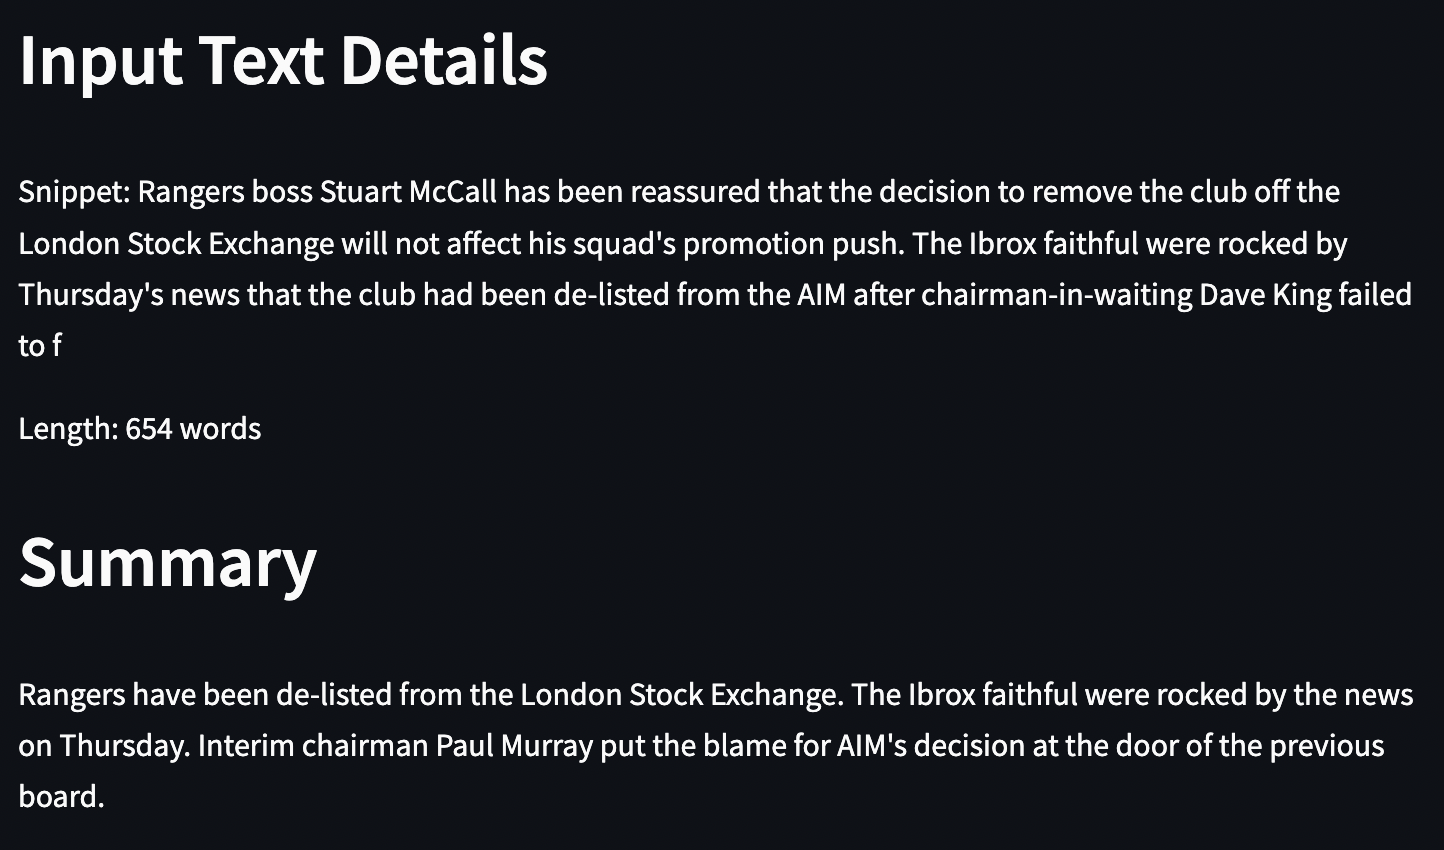
\includegraphics[width=300pt]{goodSummary.png}
    \caption{Sample Input Text and Summary}
    \label{fig:goodSummary}
\end{figure}

\begin{figure}[ht]
    \centering
    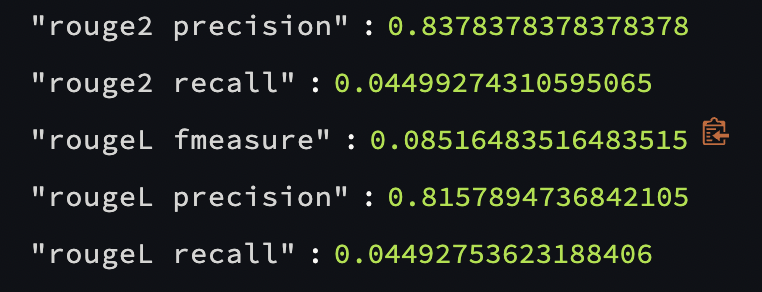
\includegraphics[width=300pt]{goodSumGoodRouge.png}
    \caption{Rouge Scores}
    \label{fig:goodSumGoodRouge}
\end{figure}

\begin{figure}[ht]
    \centering
    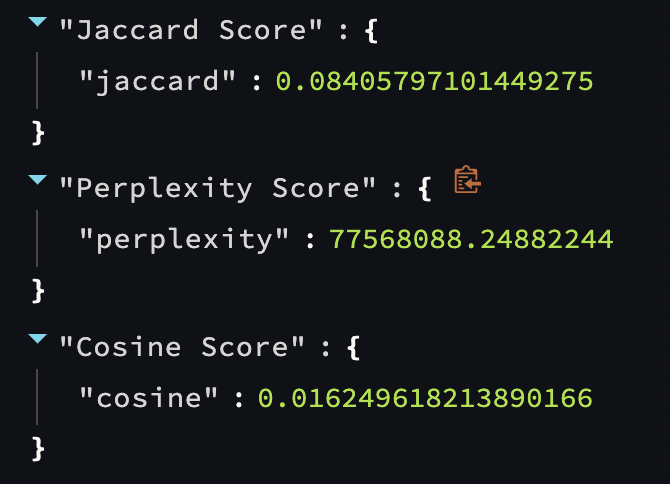
\includegraphics[width=300pt]{goodSumBadJacCos.png}
    \caption{Jaccard, Cosine, and Perplexity Scores}
    \label{fig:goodSumBadJacCos}
\end{figure}



\vspace{5pt}

However, when we look at the scores for this summary, we see a different story.
All Rouge scores support the claim that this is a good summary, as shown in fig\ref{fig:goodSumGoodRouge}.
The perplexity score (see fig\ref{fig:goodSumBadJacCos}) is extremely high, which indicates that the summary is itself vastly different from the original text.
Both the cosine similarity and Jaccard similarity scores are low (fig\ref{fig:goodSumBadJacCos}), which doesn't line up with this model's architecture.
BART specializes in extractive summarization, meaning that it snips out irrelevant text sequences and only keeps the most important ones.
When the text size differences are taken into account (as they are in our system), this model should do well on the Jaccard and cosine similarity scores.
Similarly, the perplexity score should be much lower, as the summary is a set of subset texts from the original article.
To compound the issue, the dataset that this summarization pulls from is the same one the BART model was trained on.
This is a clear example of the inconsistency between metrics. 

\vspace{5pt}

This is just an example of the many inconsistencies of text summarization models and their scoring metrics that can be found while using our tool.
We encourage the reader to try out our tool extensively to see how their assessments of the summarizations line up with the score report generated.
From this project, a few of the authors are hoping to take a deeper dive into these inconsistencies and plan to search for more clues on how model architectures play into this erroneous behavior.

\pagebreak
